 It begins! Today will be entirely tutorials---I arrived just in time for the second half of the PAC-Bayes tutorial. 

\subsection{Tutorial: PAC-Bayes Theory (Part II)}

The speakers are Benjamin Guedi and John Shawe-Taylor. \\

{\bf Part I Recap:}~\citet{shawe1997pac} carried out PAC~\cite{valiant1984theory} analysis of Bayesian estimators (also see Figure~\ref{fig:pac_bayes}. Shortly after,~\citet{mcallester1999some} presented the first {\it PAC-Bayesian} bound:

\begin{figure}
    \centering
    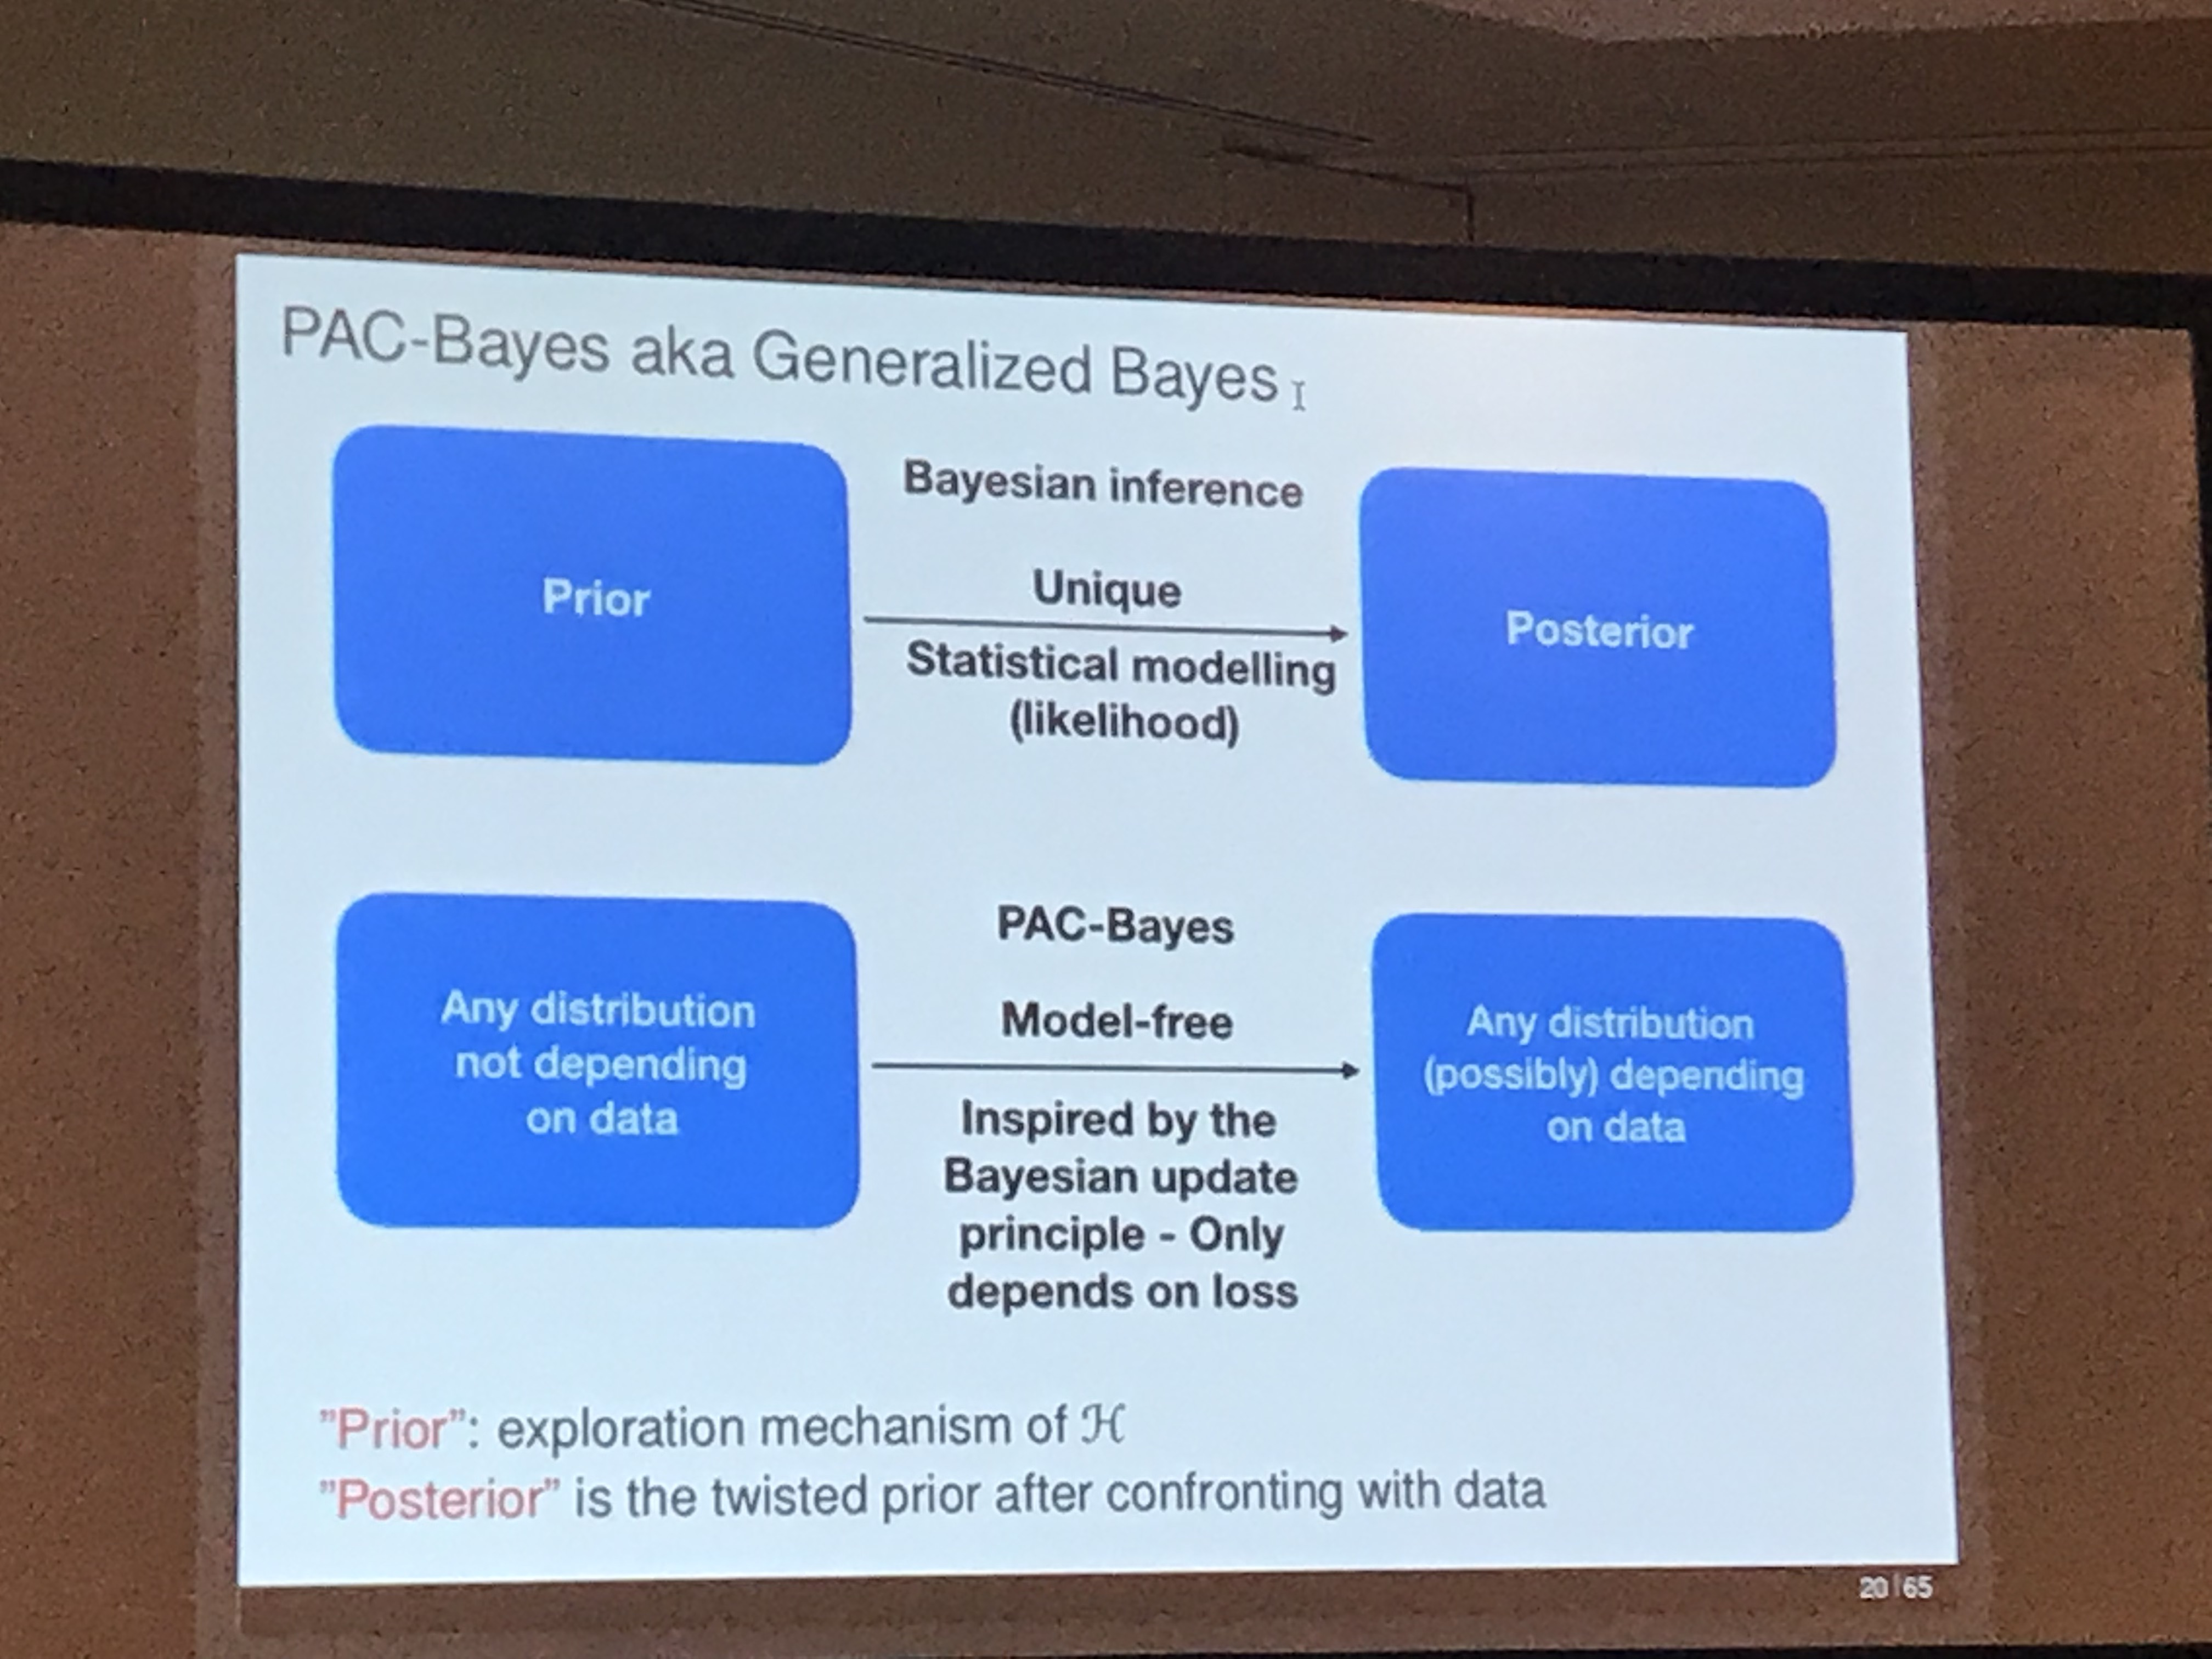
\includegraphics[width=0.5\textwidth]{images/pb1.JPG}
    \caption{Differences in Bayes and PAC-Bayes}
    \label{fig:pac_bayes}
\end{figure}


\begin{theorem}
\label{thm:pac_bayes}
(\citet{mcallester1999some}) For any prior $P$, $\delta \in (0,1]$, we have:
\begin{equation}
    \Pr\left(\forall_{Q \in \mc{H}} : R_{out}(Q) \leq R_{in}(Q) + \sqrt{\frac{\KL{Q}{P}) + \ln \frac{2 \sqrt{m}}{\delta}}{2m}}\right) \geq 1-\delta,
    \label{eq:pac_bayes}
\end{equation}
where $\mc{H}$ is the hypothesis space, $m$ is the number of samples, $R_{out}$ is the risk of a hypothesis on the test data, $R_{in}(h)$ is the risk of the data on the training data, $P$ is the prior, and $Q$ is the posterior.
\end{theorem}

PAC-Bayes: a flexible learning theoretic framework! Tight connections to regression, linear classification \& SVMs, transductive learning, uses in RL~\cite{fard2010pac}, and more.


\subsubsection{PAC-Bayes Theory}
This section explores the high level view of PAC-Bayesian Theory. \\

Q: How can PAC-Bayes drive learning? \\

A: First, recall:
\begin{equation}
    R_{out}(Q) \leq R_{in}(Q) + F(Q),
\end{equation}
Or:
\begin{equation}
    \text{Error on unseen data} \leq \text{Error on sample + complexity term}.
\end{equation}

This defines a principle strategy for obtaining new algorithms:
\begin{align}
    &h \sim Q^* \\
    &Q^* \in \text{arginf}_{Q \ll P} \left\{R_{in}(Q) + F(Q)\right\}.
\end{align}

Presents an optimization problem: can be solved or approximated to find good solutions! \\

PAC-Bayes interpretation of celebrated algorithms: 
\begin{itemize}
    \item SVM with a sigmoid loss and KL-regularized Adaboost canm be reinterpreted as minimizer of PAC-Bayesian bounds~\cite{ambroladze2007tighter}.
    \item Also, the minimizer of:
    \[
    \left\{R_{in}(Q) + \frac{KL}{\lambda}\right\},
    \]
    is the celbrated Gibbs posterior:
    \[
    Q_\lambda(h) \propto \exp(-\lambda R_{in}(h)) P9h), \hspace{5mm} \forall_{h \in \mc{H}}.
    \]
    
    When $\lambda \ra 0$, we get a flat posterior, and as $\lambda \ra \infty$, we get Dirac mass on expected risk minimization (ERMs).
\end{itemize}



\begin{theorem}
\[
\log \int (\exp \phi) dP = \sup_{Q \ll P} \left\{ \int \phi dQ - KL(Q,P)\right\}.
\]
\end{theorem}
\begin{proof}
First require variational definition of KL-Divergence~\cite{csiszar1975divergence}
\begin{align}
    -\KL{Q}{G} &= - \int \log\left(\frac{dQ}{dP} \frac{dP}{dG}\right) dQ \\
    &= -\KL{Q}{P} + \int \phi dp - \log \int(\exp \phi) dP.
\end{align}
Note that KL is non negative, $Q \ra -\KL{Q}{P}$ reaches its max in $Q=G$. Thus, taking $\phi = -\lambda R_{in}$:
\[
Q_\lambda(h) \propto \exp(-\lambda R_{in}(h)) P9h), \hspace{5mm} \forall_{h \in \mc{H}}. \qedhere
\]
\end{proof}

Q: What about non-i.i.d. data? \\

A: Sure! Let's drop the i.i.d. and bounded loss assumptions. First, consider the moment of a distribution:
\ddef{Moment}{The $p$-th moment of a distribution is given by:
\[
M_p := \int \bE\left[|R_{in}(h) - R_{out}(h)|^p )\right) dP(h).
\]}

Also make use of $f$-divergences, a generalization of the KL-Divergence. \\

\begin{theorem}
Let $\phi_p : x \mapsto x^p$. Fix $p > 1, q = \frac{p}{p-1}$ and $\delta \in (0,1)$. W/ probability at least $1-\delta$, for any distr. $Q$:
\[
|R_{out}(Q) - R_{in}(Q)| \leq (\frac{M_q}{\delta}^{1/q}(D_{\phi_{p-1}}(Q,P) + 1)^{1/p}.
\]
\end{theorem}

Takeaway: we can bound generalization error using the $f$-divergence ($D_{\phi_{p-1}}$ and moment $(M_q)$. Proof strategy requires: 1) Jensen's inequality, 2) change of measure, 3) Holder's inequality, and 4) Markov's inequality. \\

Oracle Bounds;~\citet{catoni2007pac} derived PAC-Bayesian bounds for the Gibbs posterior.

\subsubsection{PAC-Bayes and Task Awareness}

Note: PAC-Bayesian bounds express a tradeoff between empirical accuracy and a measure of complexity. \\

Q: So, how can we improve the bounds we get? How do we choose the right prior distribution so that we can 1) control complexity, and 2) ensure good performance? \\

$\ra$ So: can we choose a ``better' prior? (without looking at the test data itself?) \\

{\bf Main Idea:} use part of the data to learn how to choose a prior. \\

Can use PAC-Bayes in SVMs:
\begin{itemize}
    \item Assume prior and poster are spherical Gaussians (w/ prior centered at origin, posterirer centered at a scaling $\mu$ of unit SVM weight vector).
    \item Implies that KL term in generalization error bound is $\mu^2 / 2$ (see Theorem~\ref{thm:pac_bayes}).
    \item Can computer schochastic error of posterior distribution behaves like a soft margin, scaling $\mu$ trades between margin loss and KL.
    \item Bound holds for all $\mu$, so choose $\mu$ to optimize the bound.
\end{itemize}

Q: But how do we learn the prior for SVMs?
\begin{itemize}
    \item Bound depends on distance between prior and posterir
    \item Better prior means tighter bound
    \item Idea: learn prior $P$ with part of the data.
    \item Introduce learnt prior in the bound.
    \item Computer stochastic error with remaining data: PrPAC.
    \item Can go a step further: 1) scaling the prior in the chosen direction $\tau$-PrPAC, or 2) Adapt SVM to optimize the new bound: $\eta-$Prior SVM.
\end{itemize}

Results from the above methods for tightening the bounds: see Figure~\ref{fig:pb_results}. \\

\begin{figure}
    \centering
    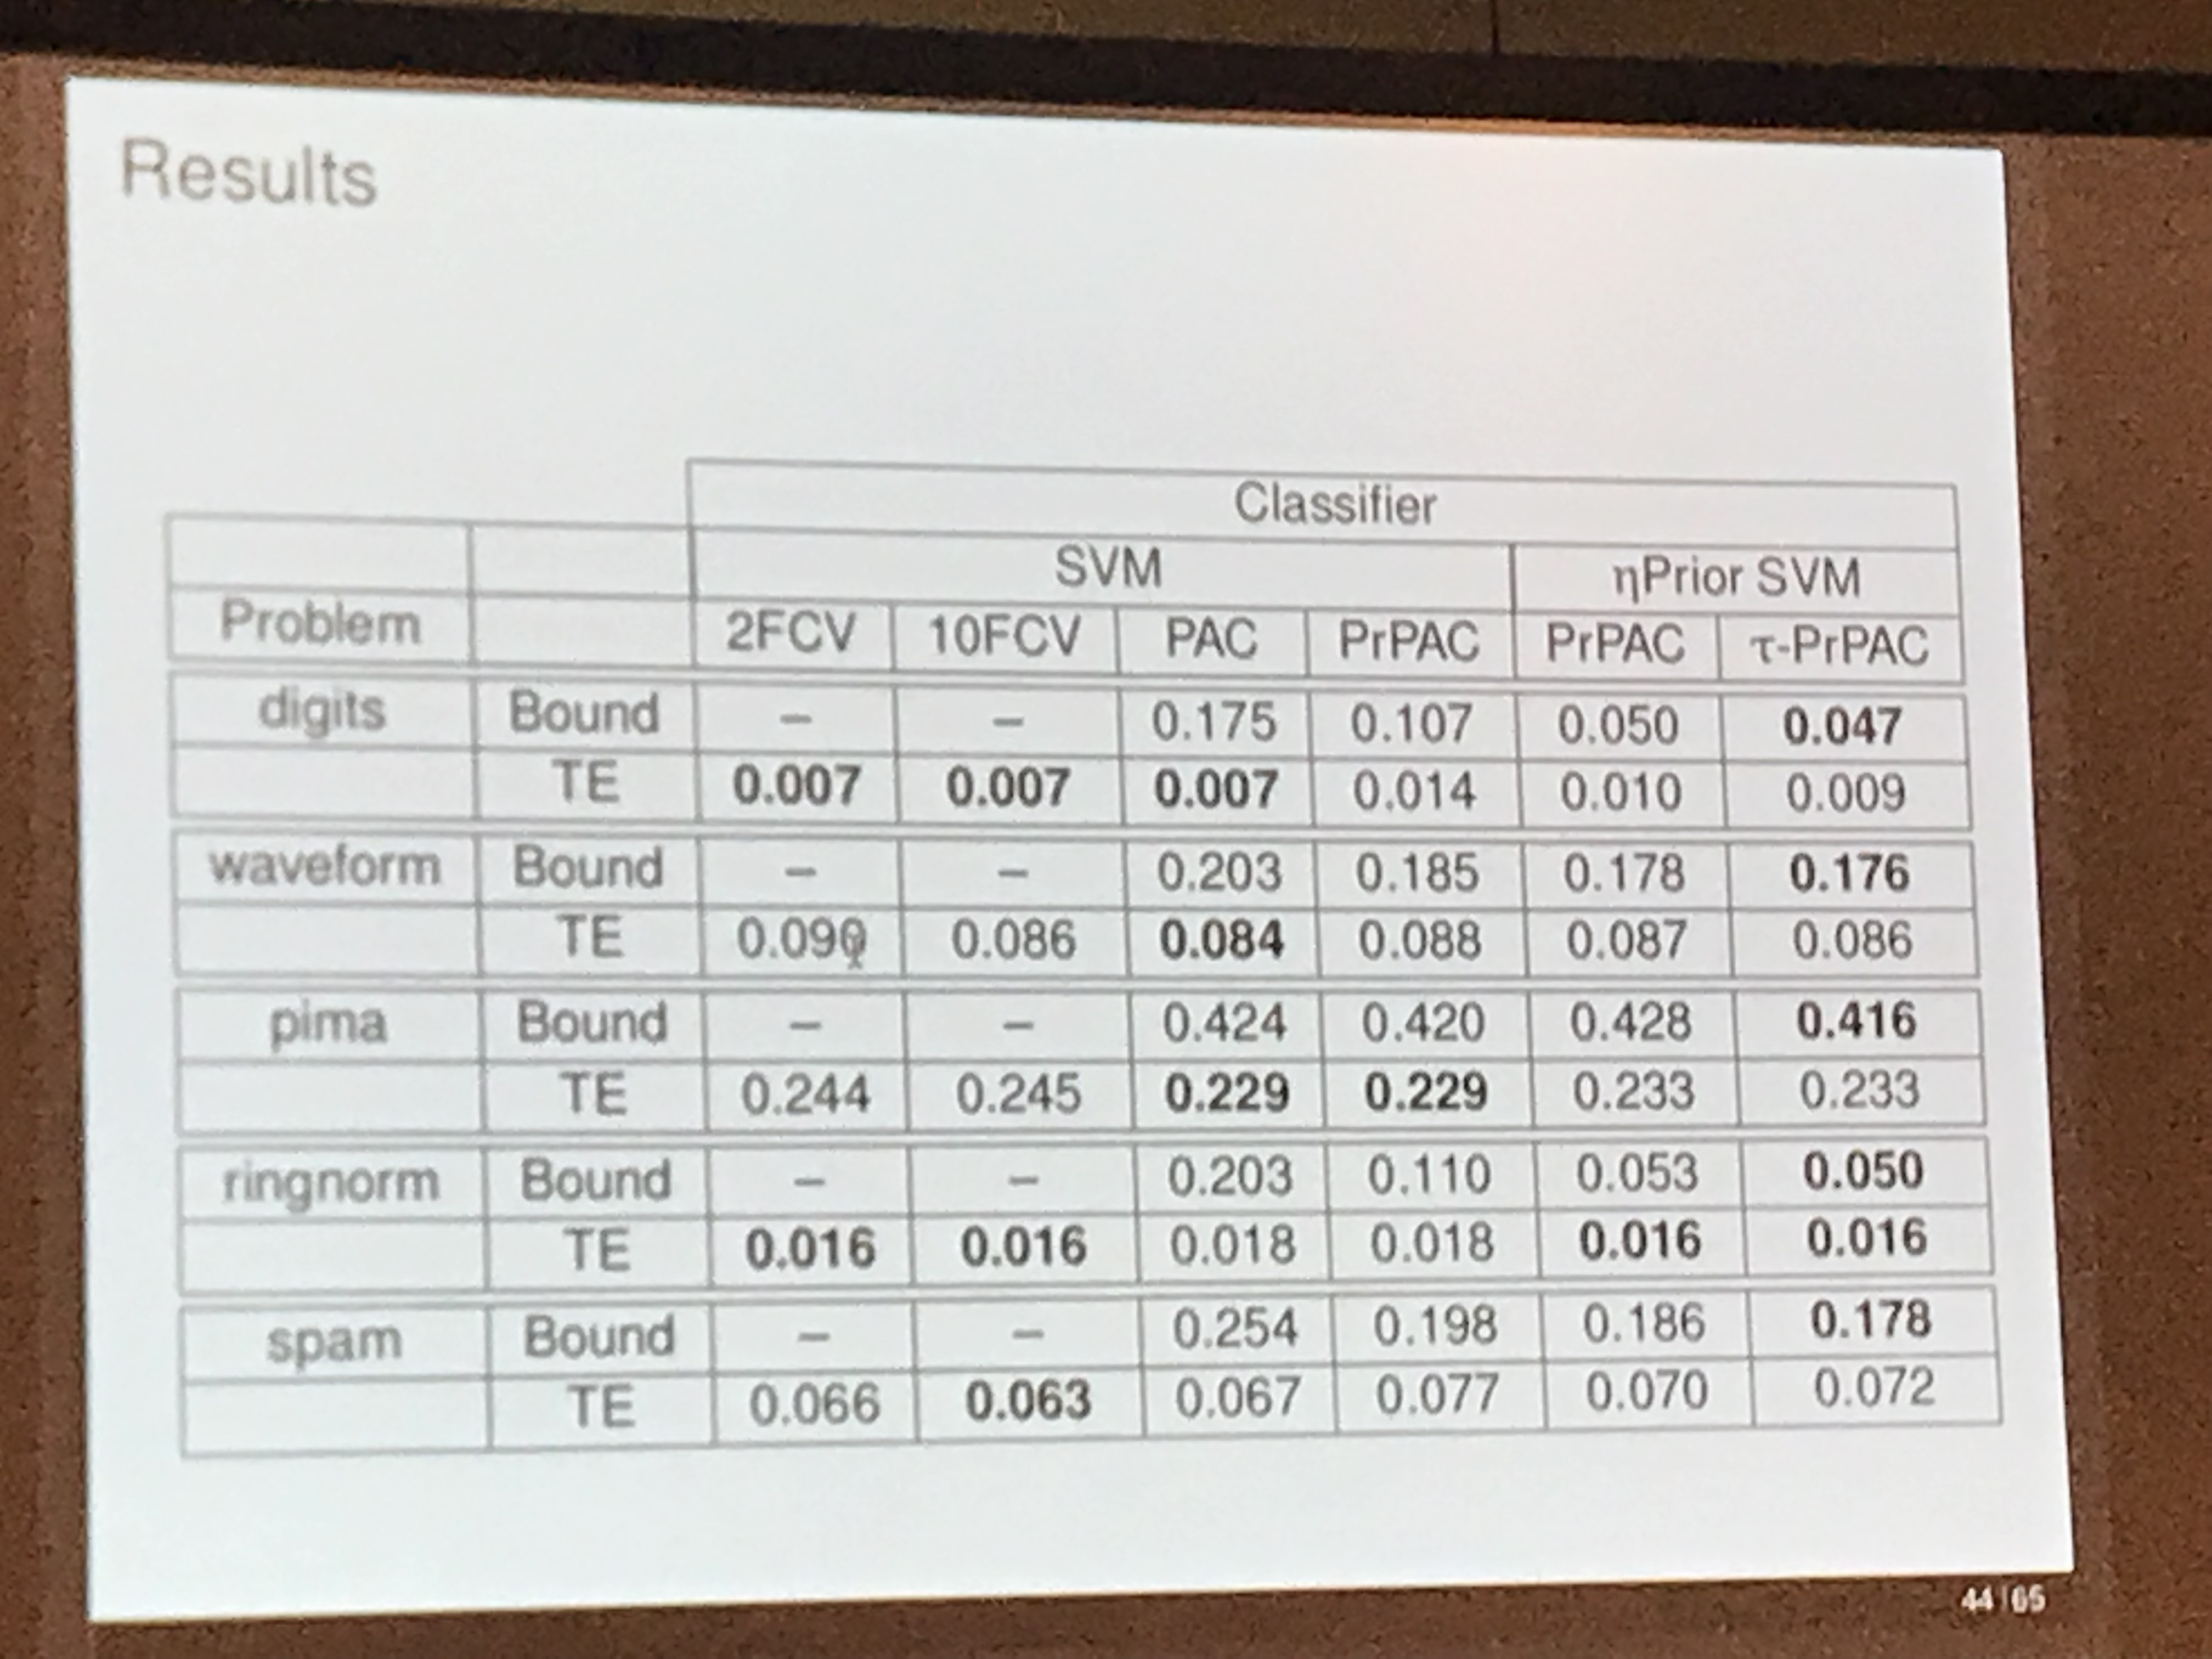
\includegraphics[width=0.5\textwidth]{images/pb_results.JPG}
    \caption{Results from applyinh differnet PAC-Bayes prior selection methods to experiments.}
    \label{fig:pb_results}
\end{figure}

Takeaways from results:
\begin{enumerate}
    \item Bounds are remarkably tight!
    \item Model-selection via these new bounds is {\it as good} as 10-fold cross validation.
    \item Best bounds don't necessarily translate into best model selection.
    
    $\ra$ We're not {\it completely} capturing the right thing (but definitely some of the right thing).
\end{enumerate}

Next up: distribution-defined priors:
\begin{itemize}
    \item Consider $P$ and $Q$ are Gibbs-Boltzmann distributions:
    \[
    P_\gamma(h) = \frac{1}{Z} \exp(-\gamma R_{out}(h) \hspace{8mm} Q_\gamma(h) = \frac{1}{Z}\exp(-\gamma R_{in}(h)).
    \]
    \item These distributions hard to work with since we can't apply it to a single weight vector. From~\citet{catoni2007pac}, we can show:
    \[
    \KL{R_{in}(Q_\lambda)}{R_{out}(Q_\lambda)} \tilde{\leq} \frac{1}{m} \left(\gamma / \sqrt{m} + \gamma^2/4m\right),
    \]
    where $\tilde{\leq}$ ignores log terms on the right hand side (\dnote{my (awful) construction for abbreviation, not theirs}).
    
\end{itemize}

On stability:
\begin{itemize}
    \item If $A$ has sensitivity $\beta$ at sample size $m$, then generalization error can be bounded~\cite{bousquet2002stability}.
    
    \item Q: Algorithm output is highly concentrated, does that imply stronger results?
    
    $\ra$ Yes! We can derive (tighter) bounds that depend on KL between a distributionally sensitive prior and a well chosen posterior.
    
    Open area! Lots of room to explore a new kind of generalization error analysis.
\end{itemize}

{\bf A final case study:} Can we use any of this to analyze deep neural networks? \\

Q: Is deep learning breaking the statistical paradigm we know? \\

$\ra$ Neural nets trained on massive datasets achieve {\it zero training error}, which does not bode well for their performance. Yet! They tend to achieve remarkably low error on test sets, too. \\

{\bf Idea:} Perhaps we can use PAC-Bayes to explain this phenomena. \\



\begin{figure}
    \centering
    \subfloat[Classical view of Overfitting]{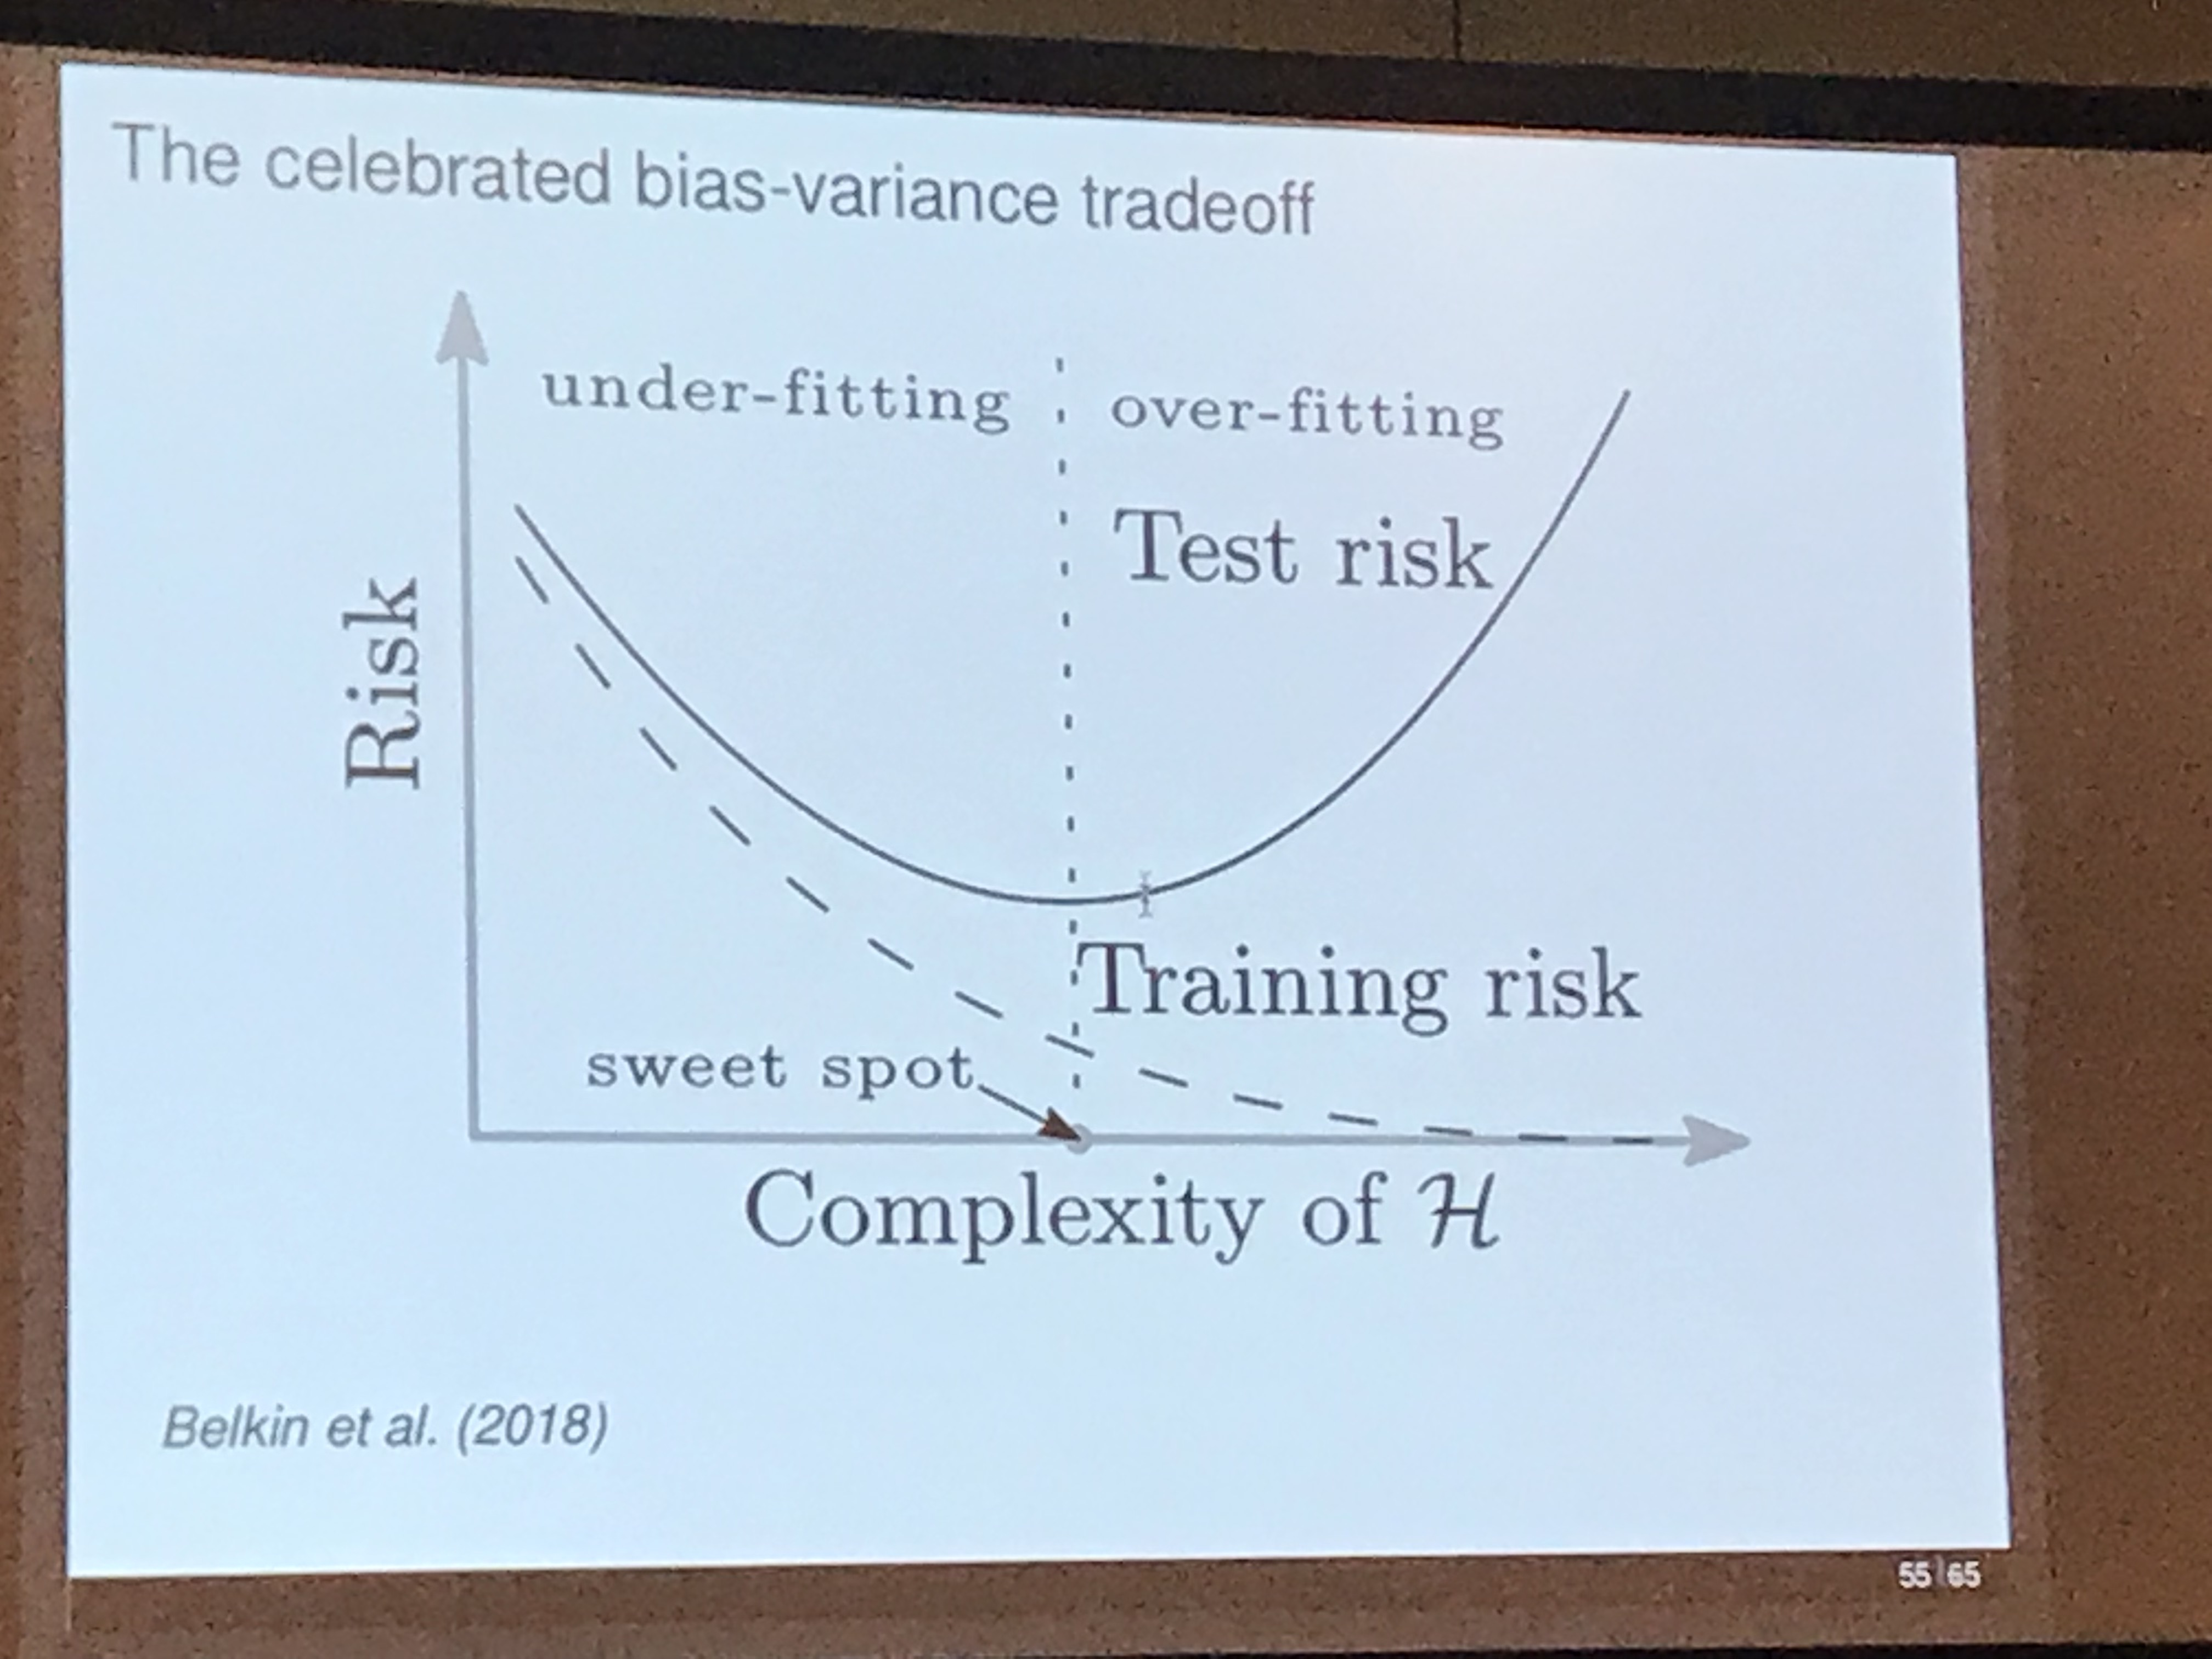
\includegraphics[width=0.45\textwidth]{images/of.JPG}} \hspace{2mm}
    \subfloat[New Paradigm?]{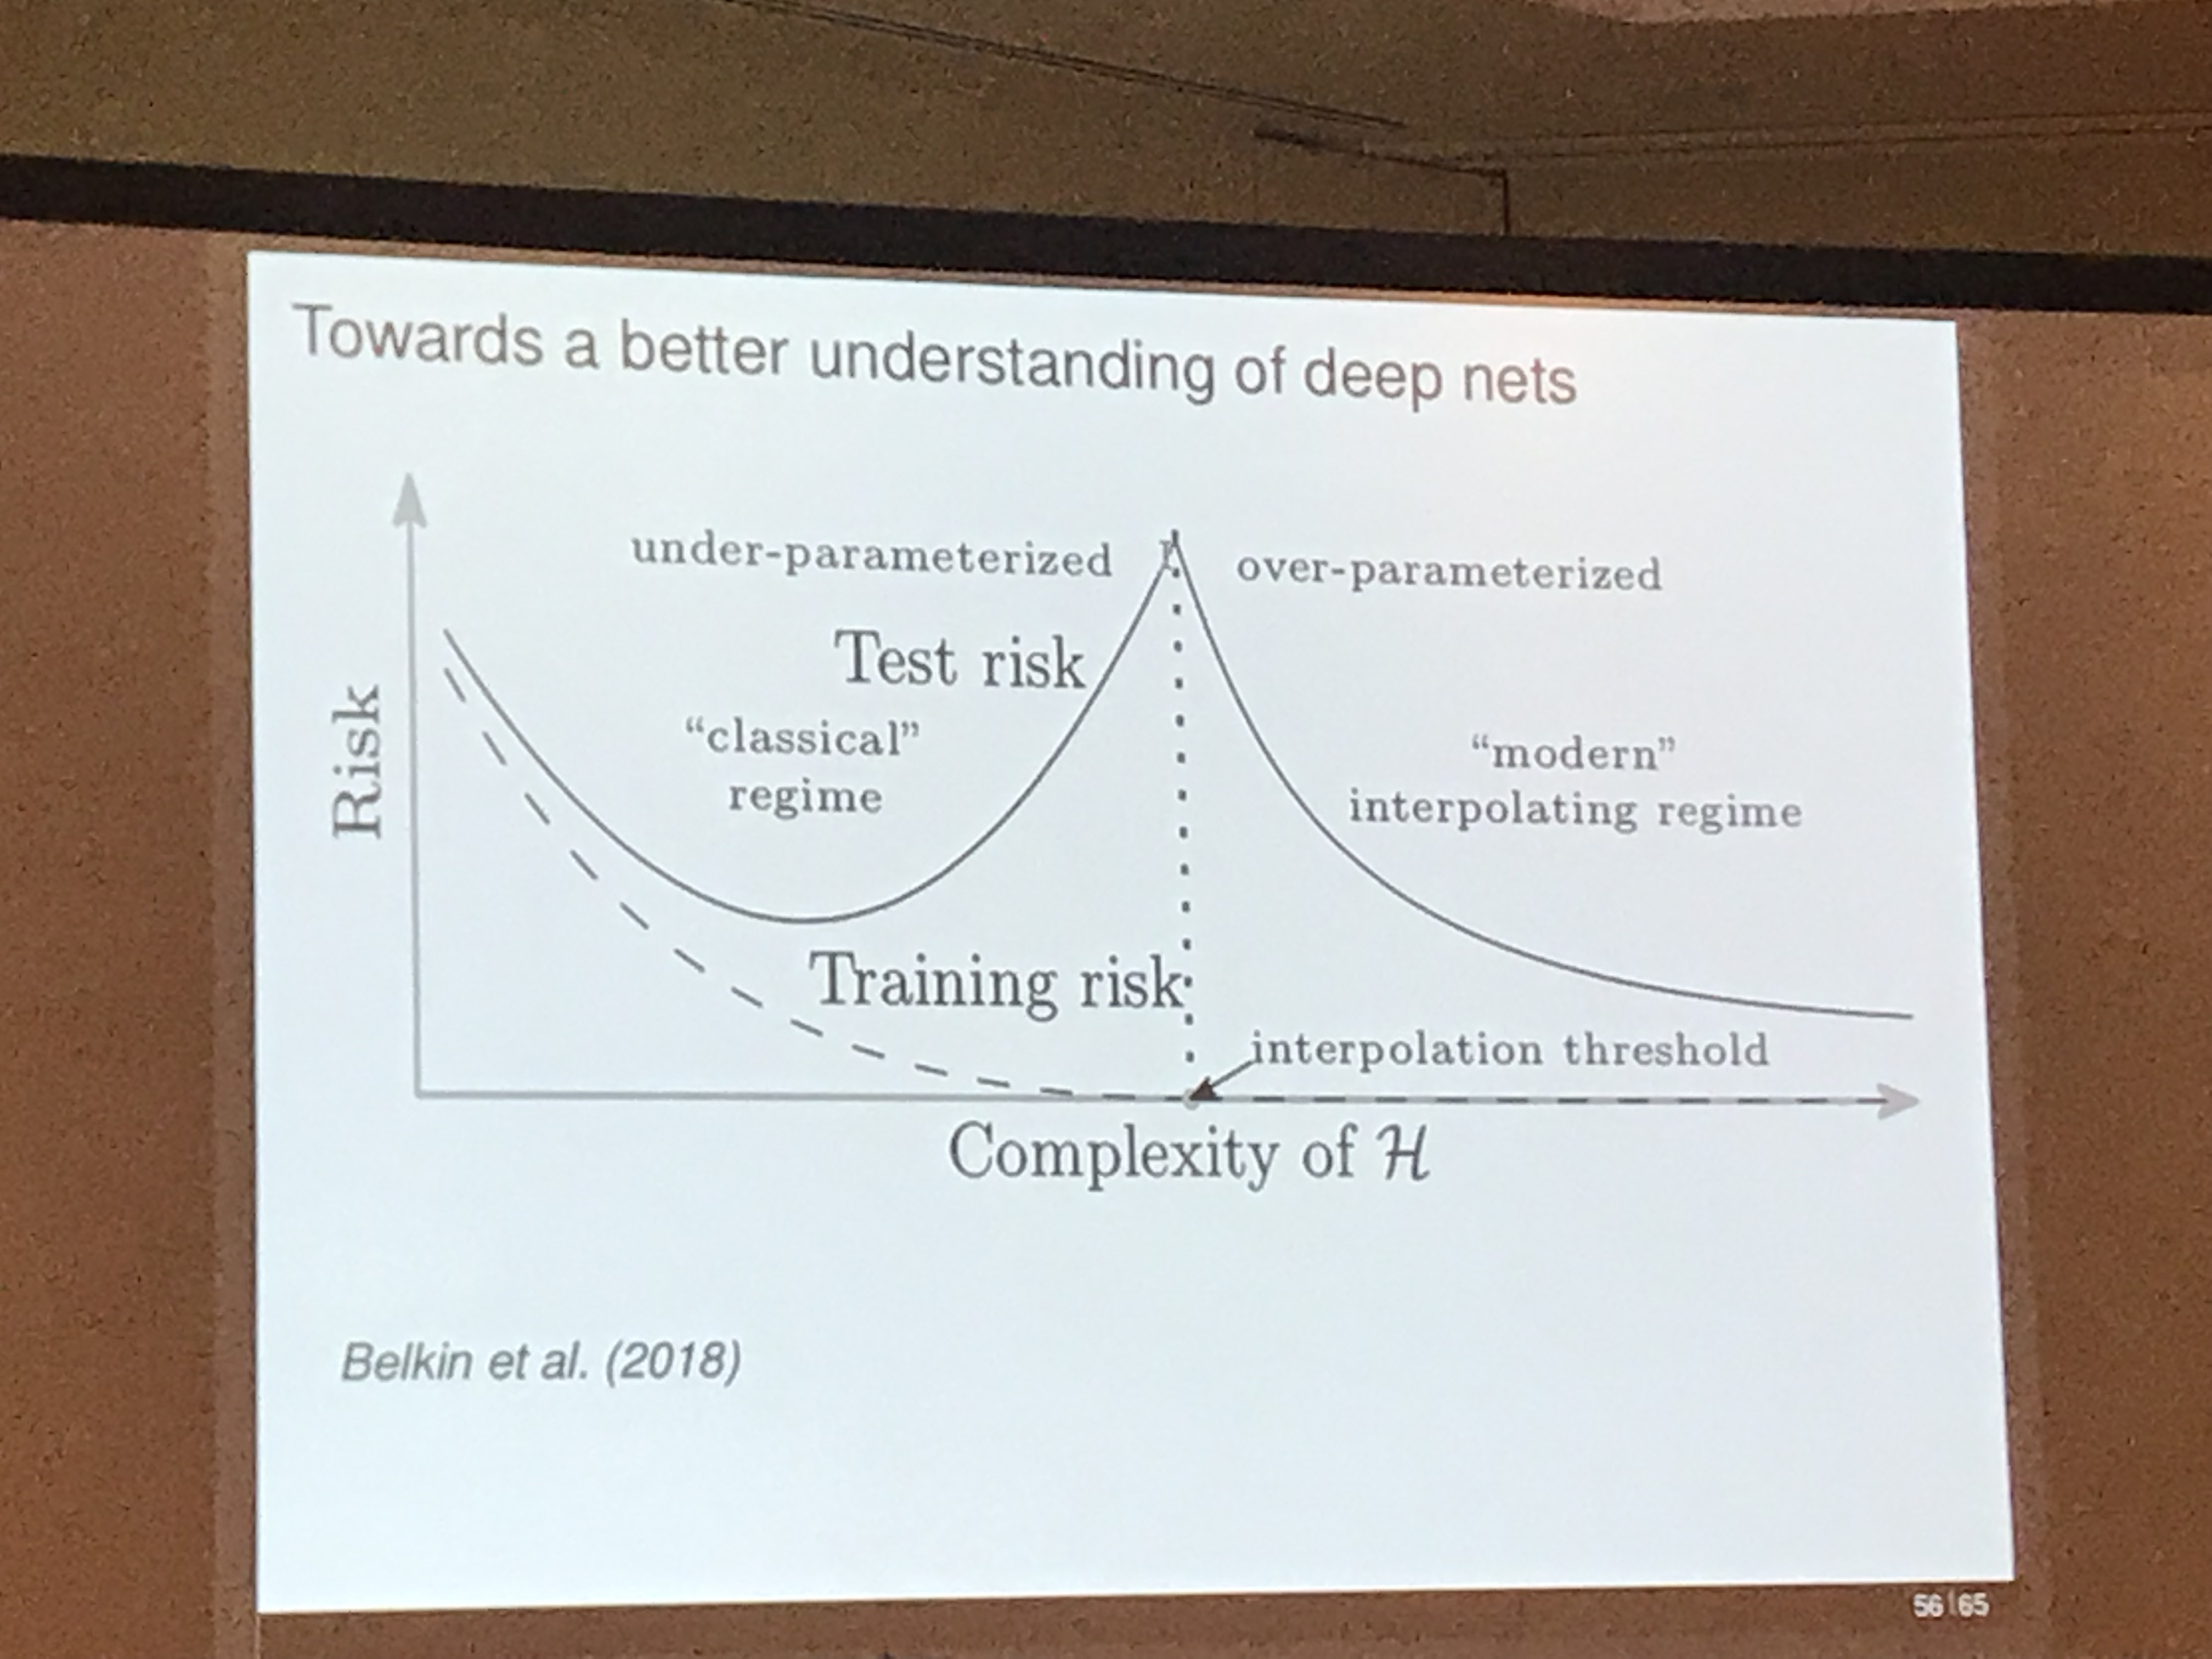
\includegraphics[width=0.45\textwidth]{images/of_2.JPG}}
    \caption{Classical view of overfitting (left), and a new proposal for why deep nets might be avoiding overfitting (right), from~\citet{belkin2018overfitting}.}
    \label{fig:overfitting}
\end{figure}

~\citet{dziugaite2017entropy} derived extremely tight deep learning generalization error bounds in this way;
\begin{itemize}
    \item Based on training to expand the ``basin of attraction"
    \item Hence, not measuring good generalization of {\it normal training}
\end{itemize}

Q: How much information is contained in the training set? \\

A1: ~\citet{achille2018information} studied the {\it amount of information} stored in the weights of deep networks. Overfitting might be related to information being stored in weights that encode training set, as opposed to the data generation distribution. \\

A2: Information bottleneck criterion~\cite{} might control this information, and could lead to a tighter PAC-Bayes bound. \\

{\bf Conclusions:}
\begin{itemize}
    \item PAC-Bayes arises from two fields: 1) statistical learning theory, and 2) Bayesian Learning
    \item Generlazies both fields and points to promising directions
    \item PAC-Bayes theory can be an inspiration toward new theoretical analysis, but also drive algorithm design (especially when theory has proven difficult).
\end{itemize}


\subsection{Tutorial: Meta-Learning}

The speakers are Chelsea Finn and Sergey Levine. \\

{\bf Motivation:} Learn from small amounts of data. \\

$\ra$ Recent advancements {\it thrive} in large diverse data sets 9in the sense that it allows for broad generalization) (see; BERT, AlexNet0 \\

$\ra$ Existing approaches require huge data sets. But, some questions:
\begin{enumerate}
\item  what if we don't have a large dataset/
\item What if we want a general purpose AI system in the world?
\item What if our data has a long tail?
\end{enumerate}

Point: these settings start to break the standard supervised learning setting. \\

Example: few shot learning with painting, people (the audience) was able to ``generalize" to guess the painter of a new painting. \\

Q: How do we accomplish this? \\

A: Well, previous experience! We weren't really doing this based on no prior experiences. We have encountered similar questions/tasks/images before. \\

Q: How might we get a machine to accomplish this task?  \\

A: Well, we might encode structure via: $\{$modeling image formation, geometry, task-specific features, hyperparameter choice$\}$, and so on \\

\dbox{{\bf Main Point:} Can we explicitly learn priors from previous experience that lead to efficient downstream learning?}

Outline:
\begin{itemize}
\item Problem statement
\item Meta-Learning Algorithms
\item Meta-Learning Applications
\item Meta-Reinforcement Learning
\end{itemize}

\subsubsection{Two Ways to View meta-Learning}

Q: How do we formulate the meta-learning problem? \\

A1: Mechanistic view! A model reads in an entire data set and makes predictions for new datapoints. Training this network uses a ``meta"-dataset which itself consists of many datasets. \\

A2: Probabilistic view: expreact prior info from a set of (meta-training) tasks that allows efficient learning of tasks. Learning a new task usis this prior training set to infer most likely posterior parameters. \\

$\ra$ A1 is more convenient for implementation, A2 is more convenient for understanding. \\

\ddef{Supervised Learning}{Find the parameters $\phi$ given data $D$:
\[
\argmax_{\phi} \Pr(\phi \mid D),
\]
where $D = \{(x_1,y_1), \ldots, (x_n, y_n)\}$. Applying Bayes rules, this comes out to:
\[
\argmax_{\phi} \log \Pr(D \mid \phi) + \Pr(\phi).
\]
}
\ddef{Meta-Learning}{Find the parameters $\theta$ that enables us to quickly solve new tasks, given a bunch of datasets $D_{\text{meta-train}}$:
\[
\argmax_{\phi} \log \Pr(\phi \mid D, D_{\text{meta-train}} = \argmax_{\theta} \log \int_\Theta \Pr(\phi \mid D, \theta) \Pr(\theta \mid D_{\text{meta-train}}.
\]
That is, we assume $\theta$ are the sufficient statistics for $\phi$. 
}
Hard to perform this decomposition in general: usually take a Maximum A Posteriori (MAP) approach. \\

{\bf Goal of Meta-Learning:} Find an appropriate set of parameters $\theta$, that are maximially probable given the meta-datasets. So:
\[
\theta^* = \argmax_\theta \log \Pr(\theta \mid D_{\text{meta-train}}.
\]

Notably, $D_{\text{meta-train}}$ might consist of {\it different} tasks (with related structure). \\

{\bf Example:} Want to classify new data sets. First, do meta learning;
\[
\theta^* = \argmax_\theta \log \Pr(\theta \mid D_{\text{meta-train}}.
\]
Then, adapt and find some nearby parameters, $\phi^*$:
\[
\phi^* = \argmax_{\phi} \log \Pr(\phi \mid D, \theta^*).
\]


{\bf Key Idea:} Our training procedure is based on a simple machine learning principle: test and train conditions much match" (from Vinyals et al. Matching Networks for One Shot learning). \\

Thus, for our above notion of meta-learning to make sense, we also need to hang on to tests {\it for each training} task. See Figure. \dnote{ADD FIG}. \\

Therefore, meta-learning can be written as:
\[
\theta^* = \max_\theta \nsum \log \Pr(\theta_i \mid D_i^{\text{test}}.
\]

\begin{figure}
    \centering
    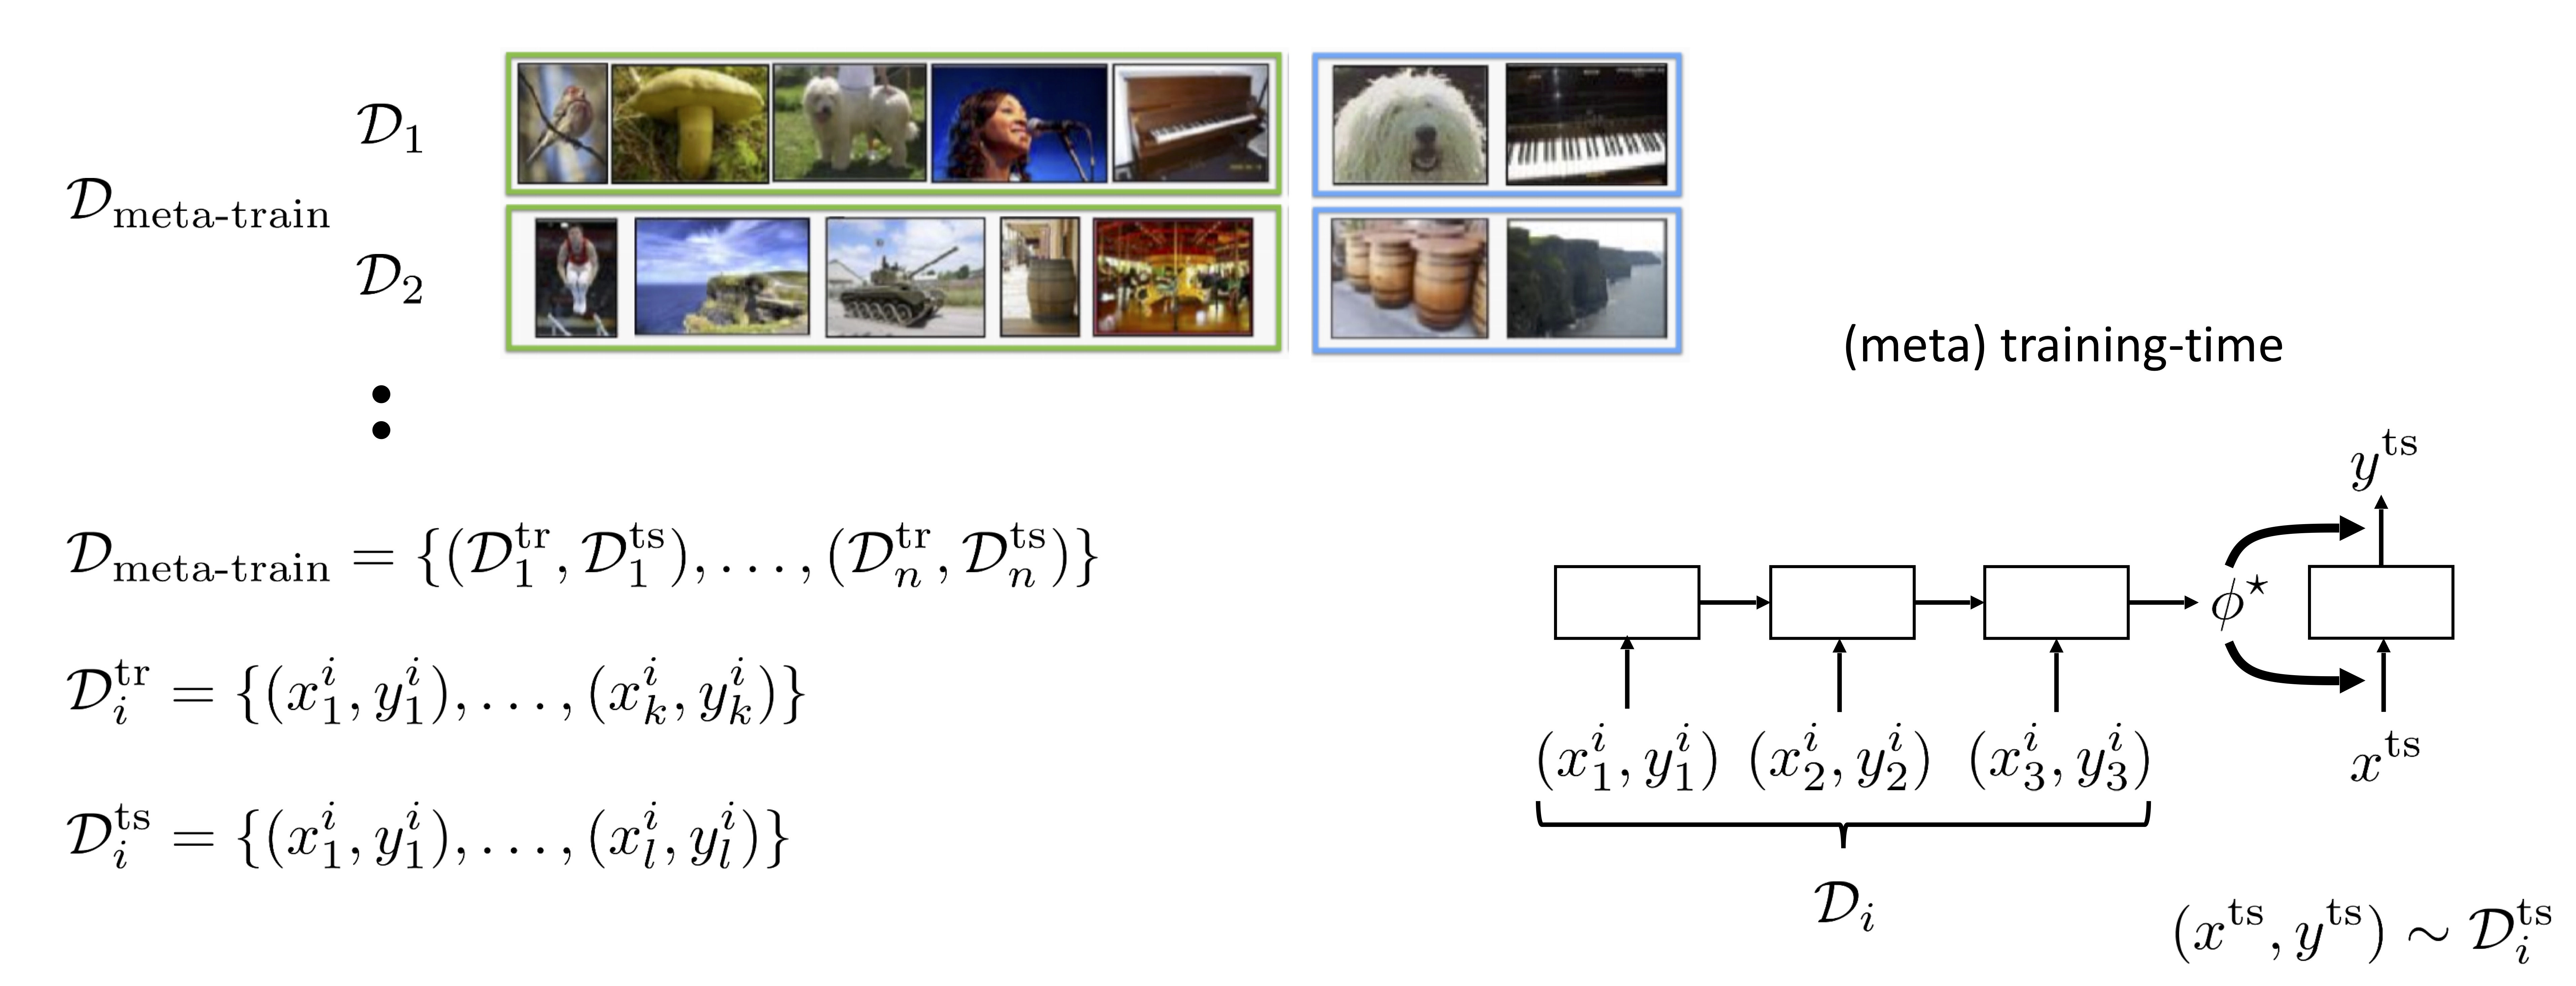
\includegraphics[width=0.75\textwidth]{images/meta_learn_1.jpg}
    \caption{Meta Learning paradigm}
    \label{fig:meta_learn}
\end{figure}

{\bf Closely related problem settings:}
\begin{enumerate}
\item Multi-task learning: special case of meta-learning where $\theta = \phi$.
\item Hyperparameter optimization: can also be cast as meta-learning with $\theta$=hyperparameters and $\phi$=network weights.
\end{enumerate}

\subsubsection{Meta-Learning Algorithms}

Before discussing algorithms, let's discuss {\it evaluation}. \\

{\bf Main Idea:} See~\citet{lake2015human}, introduced the Omniglot dataset. Idea: lots of classes, few examples of each class. Consists of 1623 characters from 50 different alphabets, 20 instances of each character. \\

$\ra$ Proposes both few-shot discriminative and few-shot generative problems. Initial few-short learning approaches w/ Bayesian models, non-parameterics. Other such databsets: CIFAR, CUB, MiniImageNEt. \\

Q: How do we evaluate a meta-learning algorithm? \\

A: Perform usual meta-training, and determine whether the resulting model can still perform quick generalization across different (held-out) tasks. \\

{\bf **General Recipe for Meta-Learning Algorithms:}
\begin{enumerate}
\item Choose a form of $\Pr(\phi_i \mid D_i^{\text{train}}, \theta)$.
\item Choose how to optimize $\theta$ with respect to max-likelihood objective using $D_{\text{meta-train}}$.
\end{enumerate}

Approach 1: Black-box adaptation. Key idea is to train a {\it neural net to represent} $\Pr(\phi_i \mid D_i^{\text{train}}, \theta)$. \\

$\ra$ For instance, might use an RNN to represent $f_\theta$, given a bunch of these meta-training datasets. Then, we can train with standard supervised learning:
\[
\max_\theta \sum_{T_i} L(f_\theta(D_i^{\text{train}}, D_i^{\text{test}})).
\]

{\bf Challenge:} Outputting all neural net parameters does not seem scalable
$\ra$ But, we don't need to output all parameters of a neural not, just the sufficient statistics. \\

Q: How can we frame this as an optimization procedure? \\

Approach 2: Acquire $\phi_i$ through optimization:
\[
\max_{\phi_i} \log \Pr(D_i^{\text{train}} \mid \phi_i) + \log \Pr(\phi_i \mid \theta).
\]
Meta-parameters $\theta$ serve as a {\it prior}. What form of prior? One form that has been successful: learn $\theta$ from {\it other tasks}. \\

{\bf Goal:} Learn a parameter vector $\theta$ that will transfer effectively, in the sense that it makes fine-tuning on new tasks easy/useful. To do so, solve the following problem;
\[
\min_\theta \sum_i L(\theta - \alpha \nabla_\theta L(\theta, D_i^{\tx{train}}), D_i^{\tx{test}}).
\]
General algorithm:
\begin{enumerate}
\item Sample task $T_i$.
\item Sample disjoint data sets from $D_i$
\item Optimize $\phi_i \la \theta - \alpha \nabla_\theta L(\theta, D_i^{\tx{tr}})$
\item Update $\theta$ using $\nabla_\theta L(\theta, D_i^{\tx{train}})$.
\end{enumerate}

So, we're left with two approaches: Optimization vs. Black-Box Adaptation \\

$\ra$ Model-Agnostic Meta-Learning (MAML), in the optimization can, can be viewed as a computation graph with embedded gradient operator (see Figure~\ref{fig:maml}:
\begin{align}
 y^{ts} &= f_{\tx{MAML}}(D_i^{\tx{train}}, x^{\tx{test}} \\
 &= f_{\phi_i}(x^{ts}),
\end{align}
where $\phi_i = \theta - \alpha \nabla_\theta L(\theta, D_i^{\tx{train}})$.

\begin{figure}
    \centering
    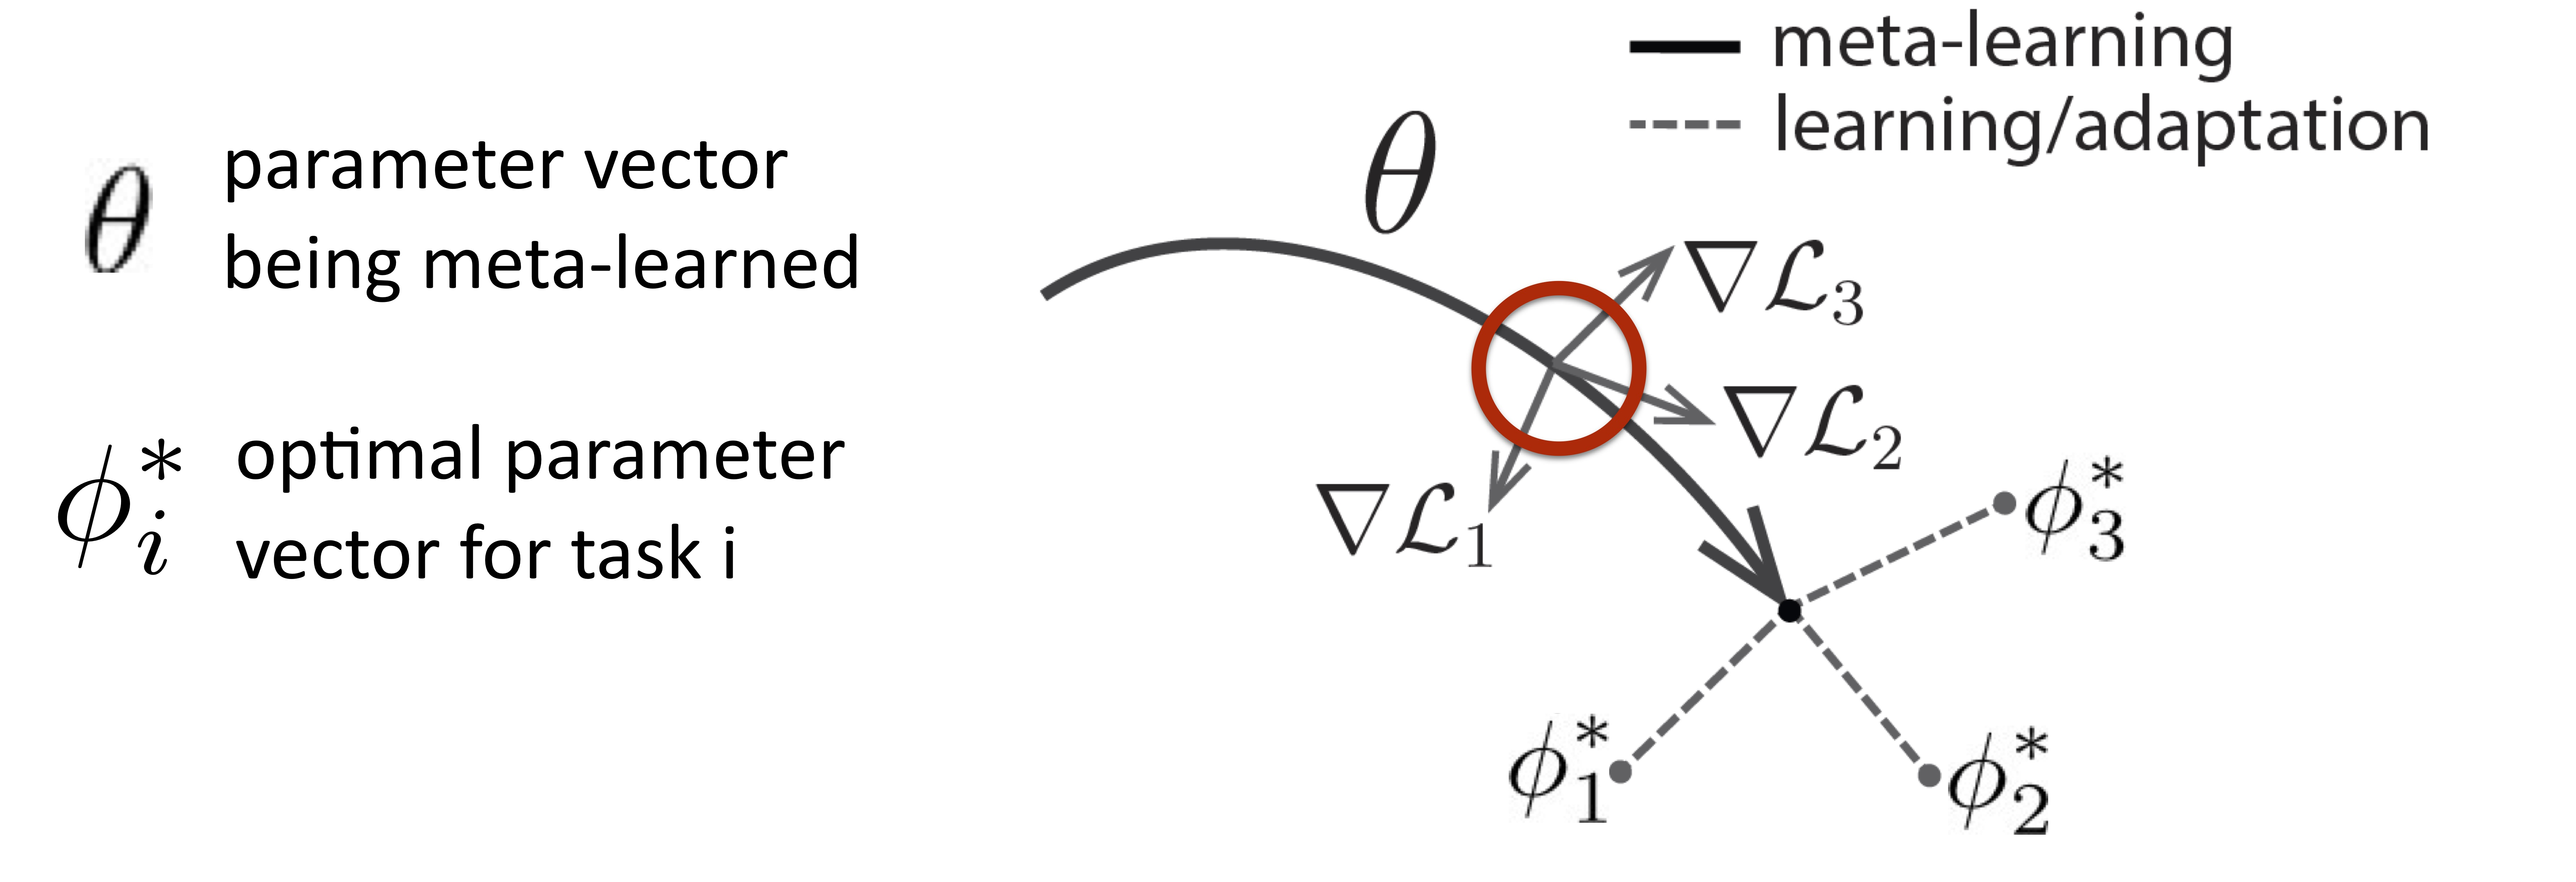
\includegraphics[width=0.65\textwidth]{images/maml.JPG}
    \caption{Model-Agnostic Meta-Learning}
    \label{fig:maml}
\end{figure}


{\bf Experiments:} Compare MAML with black-box approaches (SMAIL, MetaNetworks). Tend to find higher performance in domain adaption/extrapolated tasks. \\
$\ra$ Task was to shear digits in the Omnioglot dataset by some degree and inspect decay on performance. MAML rarely decays in performance. \\

Q: Does this learned structure come at a cost? \\

A: Not really! MAML function can approximation any function of $D_i^{\tx{train}}$, $x^{\tx{test}}$. Assumptions: nonzero $\alpha$, loss function does not lose information about the label, datapoints in $D_i^{\tx{train}}$ are unique. \\

$\therefore$ MAML has benefit of inductive bias without losing expressive power. \\

Another approach: probabilistic interpretation of optimization-based inference. Find: MAML is a form of {\it implicit} prior, roughly gradient-descent + early stopping, comes out to an implicit Gaussian prior. \\

Q; Other forms of priors expressible in meta-learning?  \\

A: Sure! Bayesian linear regression on learned features, or closed-form/convex optimization (as in ridge or logistic regression). \\


{\bf Challenges}:
\begin{itemize}
\item How do we choose an architecture that is effective for inner gradient step?
$\ra$ But, can do progressive neural search (w/ MAML) to overcome this.

\item Second-order meta-optimization can exhibit instabilities.
$\ra$ Lots of solutions available: 1) optimize only inner subset, 2) decouple learning rate, 3) introduce context variables, and so on
\end{itemize}


Approach 3: Non-parametric methods. In low data-regimes, non-parametric methods are simple and tend to work well. \\

$\ra$ During meta-test time: few shot learning $\equiv$ low data regime. During meta-training, still want to be parametric. \\

Q: Can we use parametric meta-learners that produce effectiv non-parametric learners? \\

A: Yes! Use non-parametric learners by comparing test data with training images. \\

Key Idea: learn a metric space that leads to more effective comparisons and predictions at test time. \\

%{\bf Comparison:} Compare these three approaches to meta-learning. 
{\bf Takeaways:} Each approach has some advantages/disavantages, listed in Figure~\ref{fig;maml_types}.
\begin{figure}[h!]
\centering
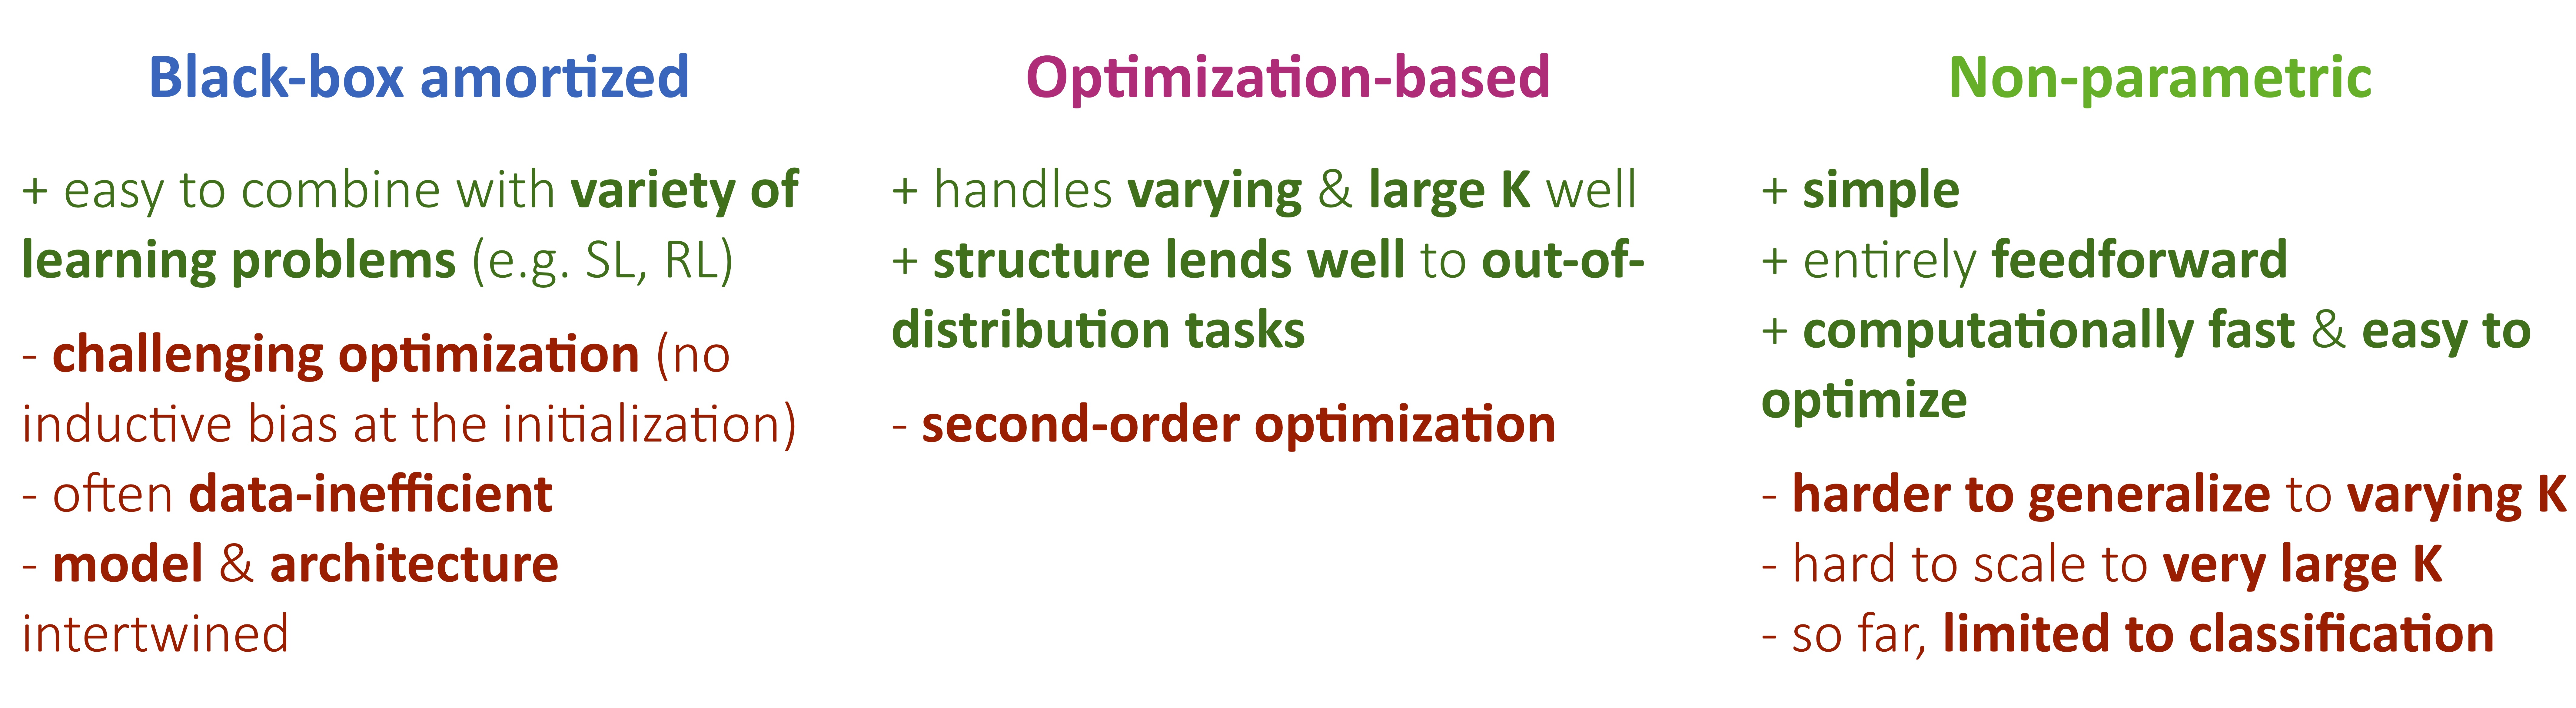
\includegraphics[width=0.85\textwidth]{images/maml_types.JPG}
\caption{Advantages and disadvantages of different approaches to meta-learning.}
\label{fig:maml_types}
\end{figure}


Approach 4: Bayesian Meta-Learning. \\

Assume we have a parameter prior $\Pr(\theta)$, $\Pr(\phi_i)$, can we sample $\phi_i \sim \Pr(\phi_i \mid x_i^{\tx{train}}, y_i^{\tx{train}})$. \\

Simple Idea: use neural net to produce a gaussian distribution over $h$, with $h$ some subset of relevant weights of the network (like the last layer). \\


Q: Okay, but what about Bayesian optimization-based meta-learning? \\

A: Sure! Lots of ways to do this. One idea is to model $\Pr(\phi_i \mid \theta)$ as Gaussian, perform variational inference for training (see Ravi and Beatson 2019). Another approach: do gradient-based inference on last layer only, use SVGD to avoid Gaussian modeling assumption (see work by~\citet{liu2016stein}). \\

$\ra$ Key Idea; Approximate $\Pr(\phi_i \mid \theta, x_i^{\tx{train}}, y_i^{\tx{train}})$ with a MAP inference. Very crude, but very convenient! \\


Further reading; ~\citet{garnelo2018conditional},~\citet{kim2018bayesian},~\citet{ravi2018amortized}.


{\bf Applications:}
\begin{itemize}
\item Vision: Few-shot image generation, image-to-image translation, generation of novel viewpoints.
\item Imitation Learning/RL: one-shot inverse RL, optimization based inference given demonstrations.
\item Language: Adapting to new programs, adapting to new languages, adapting dialogue agents to new personas.
\end{itemize}

\subsubsection{Meta-Reinforcement Learning}

Q: Why expect Meta-RL to be useful? \\

A: Well, major challenges in RL! Almost all related to the sample inefficiency of existing methods. Something TRPO, applied to a real robot, would take on the order of days or weeks for a robot to begin to make any kind of progress (in learning to walk). First, some background;\\

\ddef{Markov Decision Process (MDP)}{An MDP is a four tuple: $\langle, \mc{S}, \mc{A}, R, P\rangle$, with $\mc{S}$ a set of states, $\mc{A}$ is an action set, $P : \mc{S} \times \mc{A} \ra \Pr(\mc{S})$ denotes the transition function, and $R : \mc{S} \times \mc{A} \times \mc{S} \ra \mathbb{R}$ denotes the reward function.}

The goal is for an agent to learn a policy $\pi : \mc{S} \ra \mc{A}$ that maximizes long term expected reward:
\begin{align}
\theta^* = \argmax_\theta \bE_{\pi_\theta}\left[ R(\tau \mid \pi_\theta)\right],
\end{align}
where $\tau$ is the trajectory taken by $\pi_\theta$, and $R(\tau \mid \pi_\theta)$ picks out the rewards achieved by $\pi_\theta$. \\

``Every RL algorithm in a nutshell": finds $\pi_\theta$ either by: 1) learning a good policy directly, 2) learning a value function, or 3) learning a model and using it to find a good policy. \\

Meta-Learning so far: Learn $\theta$ uch that $\phi_i = f_\theta(D_i^{\tx{train}})$ is good for the test $D_i^{\tx{test}}$. \\

So, meta-RL problem is as follows;
\ddef{Meta-RL}{The Meta-Learning problem with the RL objective. That is, learn $\theta^*$:
\[
\theta^* = \argmax_{\theta} \nsum \bE_{\pi_{\phi_i}}\left[R(\tau \mid \pi_{\phi_i})\right],
\]
where $\phi_i = f_\theta(M_i)$}

Q: So how do we produce $M_i$, the meta-training MDPs? \\
A: One idea is to just choose related tasks (imagine we want a household chore robot, define $M_i$'s to be small and easy related tasks \\

Now, some meta-RL algorithms: similarly to supervised meta-learning, we also get a meta-RL based on black box approaches (here called ``recurrent policies"). \\

Main Question: how do we implement $f_\theta(M_i)$, with $M_i$ an MDP? Well, what should $f_\theta(M_i)$ do? \\

A: A few things: 1) improve policy with experience from $M_i$, and 2) Choose how to interact (that is, meta-RL must choose how to explore). \\

$\ra$ This mostly amounts to just running meta-RL with an RNN. \\

Q: But how do meta-RL algorithms explore effectively? This basically happens for free in this setting: optimizing reward over all episodes used in training leads to good exploration. \dnote{I don't see this, personally. Need to read more!} \\

{\bf Next View:} Treat meta-RL as an optimization problem. Standard RL formulate this as a policy gradient problem;
\[
\theta^* = \argmax_\theta \underbrace{\bE \left[R(\tau)\right]}{J(\theta)},
\]
then:
\[
\theta^{k+1} \la \theta_k + \alpha \nabla_{\theta_k} J(\theta)
\]


Next approach: meta-RL for partially observable RL! Need a richer environmental model:
\ddef{Partially Observable MDP (POMDP)}{A POMDP is a six tuple: $\langle S, A, O, P, E, r \rangle$, that is effectively an MDP, but the function $E$ generates observations from $O$ based on the current state. The agent only gets to perceive observations $o \in O$, not state.}

That is, the agent doesn't get to see everything relevant about the world, just some observation $o$ generated based on the state. \\

{\bf Key Idea:} Solving POMDPs is very hard! But, it's similar to meta-learning. Look for a policy $\pi_\theta(a \mid s, z)$, where we don't know $s$, only $z$. Works as follows: 1) Sample $z \sim \hat{p}(z_t \mid s_{1:t}, a_{1:t}, r_{1:t})$, 2) Act according to $\pi_\theta \mid s, z)$, acting as though $z$ was correct. \\


Three perspectives on Meta-RL:
\begin{enumerate}
\item Just RNN it: conceptually simple and easy, but vulnerable to overfitting and challenging to optimize.
\item MAML approach: good extraploating but complex (requires many samples).
\item POMDP approach: simple and effective, but also vulnerable to meta-overfitting.
\end{enumerate}

But: they're not that different! The POMDP approach is really just the RNN approach with an extra hidden variable, and the MAML approach is just a particular choice for the design of $f_\theta$. \\

\subsubsection{Challenges and Frontiers in Meat Learning}

Lots of exciting directions forward, but lots of challenges, too. \\

{\bf Challenge 1:} Meta-overfitting---meta learning requires a task distribution. Some approaches to meta-learning can {\it overfit} to these task distributions.\\

{\bf Challenge 2:} Task design---often these task distributions have to be chosen by hand, or are not diverse enough to encourage the right kind of behavior. It's hard to pick the task distribution in the right way! \\

{\bf Challenge 3:} Understanding which {\it algorithms} overfit---many difference approaches (black-box, optimization-based, non-parametric), but we don't have a sense of which kinds of algorithms are most vulnerable to meta-overfitting. \\

Q: What else can we do with meta-learning? \\

A1: Well, we might automatically propose tasks that generate the appropriate task distributions. $\implies$ ``Unsupervised meta learning", which refers to algorithms that learn to solve tasks efficiently without using hand-specified task distributions or labels during meta-training. \\

{\bf Challenge 4:} Memorization! Some algorithms may end up just memorizing solutions to the relevant test tasks.

{\bf Challenge 5:} How do we determine which task information should be in the input vs in the data? Broad task distributions can be useful, but makes exploration hard. If their too narrow, not representative enough. \\


\dnote{Had to run for the day!}

\spacerule